\documentclass{standalone}
\usepackage{tikz} 
\usepackage{amsmath}

\begin{document} 
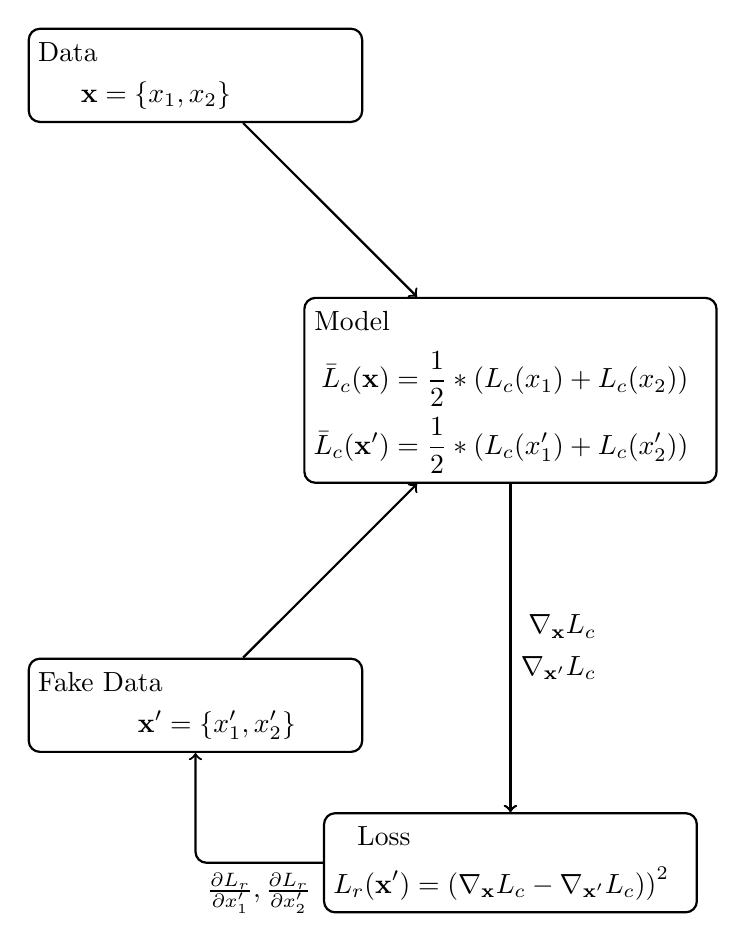
\begin{tikzpicture}[rounded corners, thick,  
    box_style/.style = {draw, rectangle, align=left}] 


    % g_i(x_i) &= \frac{\partial L_c(x_i)}{\partial w} \\
\node[box_style, text width=5cm] (2) {
    $\begin{aligned}
        \text{Model} \\
        \bar{L}_c(\mathbf{x}) &= \frac{1}{2} * (L_c(x_1) + L_c(x_2)) \\
        \bar{L}_c(\mathbf{x'}) &= \frac{1}{2} * (L_c(x'_1) + L_c(x'_2)) \\
    \end{aligned}$};

\node[box_style, below of=2, left of=2, node distance={4.0cm}, text width=4.0cm] (5)  {
    $\begin{aligned}
        \text{Fake Data} \\
        \mathbf {x'} &=\{x'_1, x'_2\}
    \end{aligned}$};

\node[box_style, above of=2, left of=2, node distance={4.0cm}, text width=4.0cm] (1) {
$\begin{aligned}
    \text{Data} \\
    \mathbf x &=\{x_1, x_2\}\\
\end{aligned}$};

\node[box_style, below of=2, node distance={6cm}, text width=4.5cm] (3) {
    $\begin{aligned}
        \text{Loss} \\
        L_r(\mathbf{x'})&= \left(\nabla_\mathbf{x} L_c - \nabla_\mathbf{x'} L_c)\right) ^2
    \end{aligned}$};

% Data to model
\draw[->] (1) -- (2); 

% Fake data to model
\draw[->] (5) -- (2);

% Model to Loss
\draw[->] (2) -- (3);

% edge label: model -> loss
\draw[->] (3) -| node[below, pos=0.25, align=left] {${\frac{\partial L_r}{\partial x_1'}, 
                                                    \frac{\partial L_r}{\partial x_2'}
                                                    }$} (5);

% edge label: model -> loss
\draw[->] (2) -- node[right, pos=0.5, align=left] {%
    $\begin{aligned}
        \nabla_\mathbf{x} L_c\\
        \nabla_\mathbf{x'} L_c
    \end{aligned}$} (3);

\end{tikzpicture} 
\end{document}